\documentclass[12pt,openany]{book}
\usepackage{lmodern}
\usepackage{setspace}
\setstretch{1.5}
\usepackage{amssymb,amsmath}
\usepackage{ifxetex,ifluatex}
\usepackage{fixltx2e} % provides \textsubscript
\ifnum 0\ifxetex 1\fi\ifluatex 1\fi=0 % if pdftex
  \usepackage[T1]{fontenc}
  \usepackage[utf8]{inputenc}
\else % if luatex or xelatex
  \ifxetex
    \usepackage{mathspec}
  \else
    \usepackage{fontspec}
  \fi
  \defaultfontfeatures{Ligatures=TeX,Scale=MatchLowercase}
\fi
% use upquote if available, for straight quotes in verbatim environments
\IfFileExists{upquote.sty}{\usepackage{upquote}}{}
% use microtype if available
\IfFileExists{microtype.sty}{%
\usepackage{microtype}
\UseMicrotypeSet[protrusion]{basicmath} % disable protrusion for tt fonts
}{}
\usepackage[left=4cm, right=3cm, top=3cm, bottom=3cm]{geometry}
\usepackage[unicode=true]{hyperref}
\hypersetup{
            pdfborder={0 0 0},
            breaklinks=true}
\urlstyle{same}  % don't use monospace font for urls
\usepackage{longtable,booktabs}
\usepackage{graphicx,grffile}
\makeatletter
\def\maxwidth{\ifdim\Gin@nat@width>\linewidth\linewidth\else\Gin@nat@width\fi}
\def\maxheight{\ifdim\Gin@nat@height>\textheight\textheight\else\Gin@nat@height\fi}
\makeatother
% Scale images if necessary, so that they will not overflow the page
% margins by default, and it is still possible to overwrite the defaults
% using explicit options in \includegraphics[width, height, ...]{}
\setkeys{Gin}{width=\maxwidth,height=\maxheight,keepaspectratio}
\IfFileExists{parskip.sty}{%
\usepackage{parskip}
}{% else
\setlength{\parindent}{0pt}
\setlength{\parskip}{6pt plus 2pt minus 1pt}
}
\setlength{\emergencystretch}{3em}  % prevent overfull lines
\providecommand{\tightlist}{%
  \setlength{\itemsep}{0pt}\setlength{\parskip}{0pt}}
\setcounter{secnumdepth}{5}
\usepackage[none]{hyphenat}
\usepackage[cmyk]{xcolor} % Recommended by US-AB
\usepackage{lmodern} % Recommended by US-AB
\usepackage{fancyhdr}
\usepackage{etoolbox}
\patchcmd{\chapter}{\thispagestyle{plain}}{\thispagestyle{fancy}}{}{} % Removes plain pagestyle from chapter headings (otherwise, page numbers are centered)
\AtBeginDocument{\addtocontents{toc}{\protect\thispagestyle{empty}}} 
\pagestyle{empty} % This makes ToC without header/footer
\usepackage[skip=15pt]{caption} % This should increase space below captions (not tested)
\raggedbottom
\usepackage[noindentafter]{titlesec}
\usepackage{titlesec}
\titleformat{\chapter}{\normalfont\bfseries}{\thechapter.}{15pt}{}\titlespacing*{\chapter}{0pt}{-50pt}{0pt}
\titleformat{\section}{\normalfont\bfseries}{\thesection.}{1em}{}\titlespacing*{\section}{0pt}{0pt}{0pt}
\titleformat{\subsection}[runin]{\normalfont\bfseries}{\thesubsection.}{1em}{}

\usepackage{CJKutf8} % For Mandarin in Acknowledgments

% For guiding quote in beginning of intro:
\makeatletter
% \renewcommand{\@chapapp}{}% Not necessary...
\newenvironment{chapquote}[2][2em]
  {\setlength{\@tempdima}{#1}%
   \def\chapquote@author{#2}%
   \parshape 1 \@tempdima \dimexpr\textwidth-2\@tempdima\relax%
   \itshape}
  {\par\normalfont\hfill--\ \chapquote@author\hspace*{\@tempdima}\par\bigskip}
\makeatother
\usepackage{placeins}
\usepackage{titlesec}

\author{}
\date{\vspace{-2.5em}}

\begin{document}

{
\setcounter{tocdepth}{3}
\tableofcontents
}
\cleardoublepage
\pagestyle{fancy} \fancyhf{} \renewcommand{\headrulewidth}{0pt}
\fancyfoot[LE,RO]{\thepage} \renewcommand{\floatpagefraction}{.9}
\setcounter{page}{9}

\chapter*{Abbreviations}\label{abbreviations}
\addcontentsline{toc}{chapter}{Abbreviations}

\begin{tabular}{ll}
\toprule
Abbreviation & Term\\
\midrule
RPF & Ribosome Protected Fragment\\
\bottomrule
\end{tabular}

\chapter{Introduction}

\section{Cancer}

According to data from the World Cancer Research Fund, in 2018 there
were an estimated 18 million cancer cases worldwide of which 9.5 in men
and 8.5 in women. Lung and breast were the most common cancers overall.
However, the most common cancers among women were breast, colorectal and
lung whereas for men these were lung, prostate and colorectal cancer.

Cancer is a disease in which cells start growing abnormally and evade
mechanisms monitoring cellular integrity. Hanahan et al. (Hanahan \&
Weinberg, 2011) summarised such mechanisms and how cancer evades them as
the hallmarks of cancer. These hallmarks will be discussed in section
xxx.

In this thesis I will discuss two studies in which breast cancer and
pancreatic cancer play a central role. Therefore in the next two
sections will focus on these two very different cancers.

\subsection{Breastcancer}

some text ater the subsection. some more text after the subsection. some
text ater the subsection. some more text after the subsection. some text
ater the subsection. some more text after the subsection.

\subsection{Pancreatic cancer}

stats and explanation on pancreatic cancer

\subsection{Hallmarks of cancer}

Hallmarks of cancer and lead into gene expression

\begin{figure}
  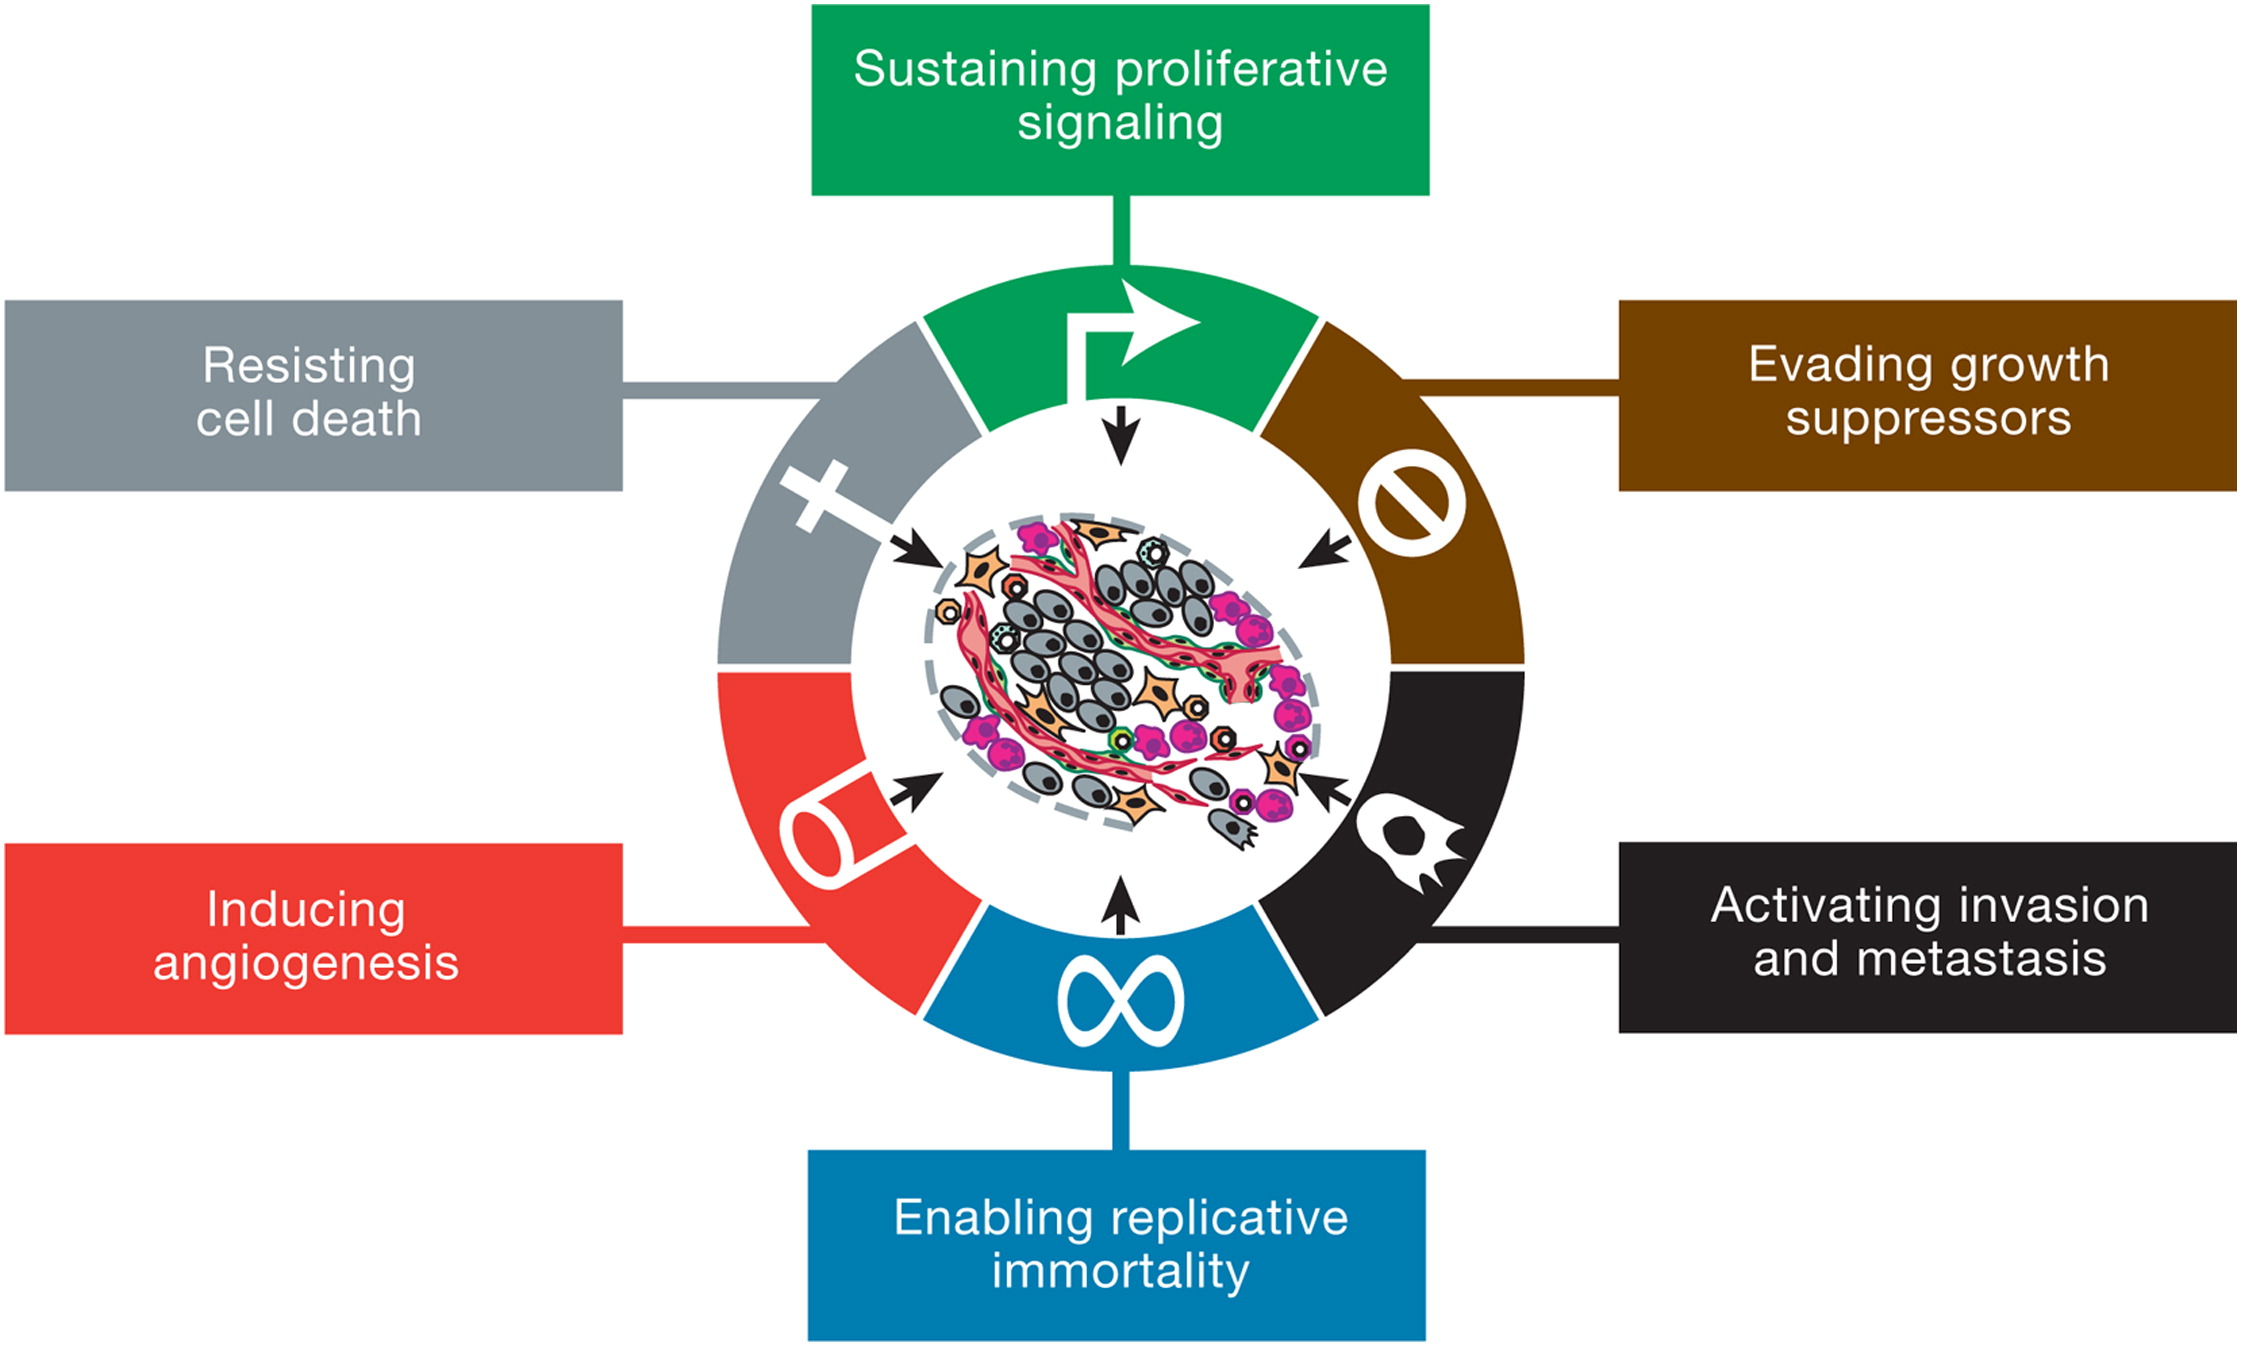
\includegraphics{./figures/hallmarks.jpg}
  \caption{The Hallmarks of Cancer - This illustration encompasses the six hallmark capabilities originally proposed in our 2000 perspective. The past decade has witnessed remarkable progress toward understanding the mechanistic underpinnings of each hallmark. 
  Reprinted from Hallmarks of cancer: The next generation, 144, Hanahan, Douglas and Weinberg, Robert A., Hallmarks of cancer: The next generation, 646-674, Copyright (2011), with permission from Elsevier \label{HOC}}
\end{figure}

\section{Central dogma of gene expression}

\section{mRNA translation}

For the vast majority of protein coding mRNAs,eukaryotic mRNA
translation occurs in the cytoplasm, however a small subset of mRNAs is
translated in the mitochondria. mRNA translation is a process that
includes initiation, elongation, termination and ribosome recycling and
is an essential process. mRNA translation inititiation is commonly
regarded as the rate limiting step. Nevertheless, regulation of mRNA
translation is also regulated at the elongation and termination phases
to a lesser extent.

\subsection{mRNA translation initiation}

In eukaryotes most mRNAs are translated by scanning the mRNA for a start
codon (AUG). This mechanism begins with the formation of the 43s
pre-initiation complex (PIC) consisting of methionyl-initiator tRNA
(met-tRNAi) in a ternary complex (TC) with guanosine triphosphate (GTP)
bound eukaryotic initiation factor 2 (eIF2). The PIC is recruited to the
5'-cap of mRNAs which is facilitatedby the eIF4F 5'-cap binding complex,
a complex consisting of eIF4E (cap binding protein), eIF4A (RNA
helicase) and eIF4G (scaffolding protein). The PIC then scans along the
mRNA from the 5' end until it encounters an AUG codon. After AUG
recognition eIF2-GTP is hydrolyzed forming a stable 48S PIC.
Afterrelease of eIF2-GTP the 60S ribosomal subunit joins to form the 80S
ribosome and protein synthesis can commence(Hinnebusch, 2014,Dever \&
Green (2012)). Next to this scanning mechanism, mRNA translation can
also be initiated via alternative cap independent mechanisms(Wurth \&
Gebauer, 2015).

\subsection{mRNA translation elongation}

The 80S ribosome contains three sites; the acceptor (A), peptidyl (P)
and Exit (E) sites. After initiation, the 80S ribosome is positioned
with the met-tRNAi in the P site at the AUG codon with the following
codon of the transcript in the A site awaiting its cognate tRNA. The
tRNA arrives in a TC together with eukaryotic elongation factor
1A(eEF1A)at the A-site of the ribosome. After arrival in the A-site,the
codon is then recognized. The binding of eEF1A is GTP dependent,
recognition of the cognate codon by the tRNA triggers hydrolysis whereby
eEF1A releases from the tRNA thatis then recycled by eEF1B.Peptide bonds
are then formed accompanied by a tRNA hybrid state whereby acceptor
sites of tRNAs in the A-and P-site now move to the P-and E-site. Binding
of eEF2-GTP then promotes translocation of the tRNAs into the P-and
E-sites after which eEF2B-GDP releases. After release of the deacylated
tRNA from the E-site the ribosome is ready for the next cycle. This
process is repeated until a stop codon (UAA,UGA or UAG)is detected by
the ribosome(Dever \& Green, 2012). mRNA translation termination
Termination of mRNA translation is facilitated by two release factors,
eRF2 and eRF3-GTP. The TC with eRF2 and eRF3-GTP binds to the A-site of
the ribosome. Recognition of the stop codon by the ribosome then causes
hydrolysis resulting in a conformational change and release of the
polypeptide. eRF1 and the ATP binding cassette protein (ABCE1) together
promote the splitting of the 60S and 40S subunits, of which the 40S
subunits has still bound tRNA. After release of the tRNA from the 40S
subunits the parts of the translational machinery can be recycled(Dever
\& Green, 2012).

\section{Regulation of mRNA translation}

\subsection{mTOR singalling pathway}

mTOR is a conserved Ser/Thr kinase and is found in two structurally and
functionally distinct complexes, mTORC1 and mTORC2. mTORC1 contains
mTOR, regulatory associated protein of TOR (raptor), the GTPase
beta-subunit like protein (GbetaL) and disheveled, EGL-10, pleckstrin
{[}DEP{]} domain containing mTOR-interacting protein (deptor). mLST8 and
deptor are found in both mTORC1 and mTORC2.However,
rapamycin-insensitive companion of TOR (rictor), mammalian
stress-activated protein kinase {[}SAPK{]}-interacting protein (mSIN1),
and proline-rich protein 5 (protor) are specific to
mTORC2({\textbf{???}},Pearce et al. (2007)). In regards to regulation of
mRNA translation, mTORC1 is a key player in regulation of translation
initiation through facilitating the release of eIF4E from 4E-BPsvia
phosphorylation of 4E-BPs by mTOR (Hsieh et al., 2010). Furthermore,
substrates of mTORC1 include ribosomal S6 kinases (S6Ks) 1 and
2(Schepetilnikov et al., 2013), and La ribonucleoprotein domain family
member 1 (LARP1)(Tcherkezian et al., 2014). mTORC2 is found to associate
with ribosomes to promote co-translational phosphorylation and
foldingofnascent Aktpolypeptide(Oh et al., 2010).As mentioned mTORC1 is
activated via growth hormonesincludinginsulin and insulin like growth
factor (IGF).For example,wheninsulin binds to the insulin
receptor,tyrosine kinases (RTKs) and phosphoinositide 3-kinase (PI3K)
are activated. Phosphatidylinositol 3,4,5-triphosphate (PIP3) is then
generated by PI3K from Phosphatidylinositol 4,5-biphoasphate (PIP2).
This step is reversed by PTEN which hydrolyzes PIP3 to PIP2, thereby
working antagonistically to PI3K. PIP3 recruits AKT and
phosphoinositide-dependent kinase1 (PDK1) towards the plasma membrane
where AKT is phosphorylated by PDK1. Ras homologue enriched in brain
(Rheb) is a GTPase that stimulates mTOR in its GTP bound form. The
tuberous sclerosis complex (TSC) consists of TSC1 (scaffold protein) and
TSC2 is a GTPase-activating protein (GAP) which inhibits Rheb through
hydrolysis of Rheb-GTP to Rheb-GDP, thereby inhibiting mTOR activity.
AKT mediates phosphorylation of TSC2, leading to a decreased GAP
activity and reduced mTOR inhibition. Signaling through the Ras GTPase
by growth factors may also activate mTORC1 through the RAF/MEK/ERK axis
whereby extracellular signal-regulated kinase (ERK) leads to direct
phosphorylation of TSC2 and raptor or via the RSKs(Roux \& Topisirovic,
2018,Roux \& Topisirovic (2012),Laplante \& Sabatini (2012)).Protein
synthesis is the most energy expensive process within cells(Buttgereit
\& Brand, 1995).Therefore,regulation of mRNA translation is tied to
cellular energy levels. AMP-activated protein kinase (AMPK) is a kinase
activated by increased AMP/ATPratioas well as ADP/ATP ratios. AMPK
inhibits protein synthesis by activation of TSC2, thereby reducing mTOR
activity. Furthermore, cellular oxygen levels are linked to ATP
production, where low oxygen levels reduce ATP production leading to
AMPK activation(Leibovitch \& Topisirovic, 2018).mTOR modulates global
mRNA translation mainly throughmodulation of 4E-BPs and S6Ks(Bruno D.
Fonseca et al., 2014,Hay \& Sonenberg (2004)). However,mTOR also
mediates selectivemRNA translation (Gandin et al., 2016). Upon
activation, mTORphosphorylates 4E-BPsleading to release of eIF4E(Roux \&
Topisirovic, 2018,Saxton \& Sabatini (2017)). As described above eIF4E
then facilitates assembly of eIF4F, whichis essential for cap dependent
mRNA translation initiation. S6Ks (S6K1 and S6K2) phosphorylates
multiple componentof the translational machinery such as RPS6which is
implicated in ribosome biogenesis(B. Magnuson, Ekim, \& Fingar, 2012).
Furthermore, S6Ks also phosphorylateeEF2 kinase which is a negative
regulator of protein synthesis(X. Wang et al., 2001).Lastly, S6Ks
phosphorylate programmed cell death 4 (PDCD4)triggering its
SCFbetaTrCP-dependent degradation (Carayol et al., 2008).PDCD4is a
factor blocking the eIF4A-eIF4G interactionby binding to eIF4A.Binding
of PDCD4 to eIF4A leads to inhibitionof eIF4A activity and thus
translation of mRNAsthat require RNA helicase activity(Yang et al.,
2003). More recent work indicates an effect of mTORC1on LA motif
(LAM)-containing factor family La-related protein 1 (LARP1). In that
study theconserved RNA-binding protein of LARP1interacts with raptor and
is phosphorylated by mTORC1.However, the scope of LARP1 mediated
effectsremaincontroversial.It has been suggested LARP1 stabilizes or
regulates translation of mRNAs with the terminal oligo pyrimidine (TOP)
motif in a context dependent manner{[}Tcherkezian et al. (2014),Bruno D
Fonseca et al. (2015),Deragon \& Bousquet-Antonelli (2015)).

\subsection{The integrated stress response}

eIF2 delivers Met-tRNAi to the 40s ribosomal subunit (33). During the
integrated stress response (ISR) the alpha subunit of eIF2 is
phosphorylated on Ser51 which leads to a global suppression of 5' cap
dependent mRNA translation. Upon eIF2alpha phosphorylation, eIF2alpha
directly engages the guanine nucleotide exchange factor eIF2beta.
eIF2beta converts the inactive eIF2-GDP to eIF2-GTP, therefore eIF2alpha
phosphorylation limits eIF2 recycling of Met-tRNAi to the ribosome (33).
Simultaneously, eIF2alpha phosphorylation stimulates selective
translation of mRNAs with upstream open reading frames (uORFs) such as
ATF4 which is a transcription factor that plays a crucial role in the
adaptation to stress (34). There are multiple kinases, activated
depending on the cellular stress, which phosphorylate eIF2alpha. These
kinases include Protein kinase R-like endoplasmic reticulum kinase
(PERK) which is activated by misfolded peptides in the endoplasmatic
reticulum (ER), Heme regulated eIF2alpha kinase (HRI) which is activated
during oxidative stress, protein kinase R (PKR) which is activated in
response to certain viral infections and GCN2 which is activated when
cells are deprived of amino acids (4, 35--37). Therefore, several
distinct stress origins converge on the same pathway regulating mRNA
translation.

\subsection{REGULATION OF TRANSLATION THROUGH 5’ AND 3’ UTR STRUCTURES AND ELEMENTS}

Recruitment of the PIC to the 5' UTR is followed by scanning until
recognition of a start codon. During scanning a process called leaky
scanning can occur where the first encountered AUG is not recognized due
to sub-optimal sequences flanking the start codon. Leaky scanning is
influenced by eukaryotic elongation factors (eEF) 1 and eEF5 where high
levels of eEF1 promote leaky scanning and blocking of non-cognate
initiation whereas eEF5 works antagonistically to eEF1. Nonetheless,
translation is most favorably initiated when an AUG is encountered with
the ``Kozak'' context. Near cognate triplets e.g.~NUG can also initiate
translation at a much lower frequency as compared to cognate triplets
(10). Structures in the 5' UTRs can influence translation initiation
e.g.~stem loops (SL) like the iron responsive element (IRE), which
regulates translation of mRNAs involved in iron homeostasis depending on
iron availability (38) and RNA G-quadruplexes which block scanning (39).
Therefore, the degree of structure of a 5' UTR can be an indicator
whether an mRNA's translation efficiency is regulated or not. In
eukaryotes the vast majority of mRNAs have 5' UTRs with a median length
ranging from 53 to 218 nucleotides, where humans have 5' UTRs with the
longest median length. Furthermore, mRNAs with long and structured 5'
UTRs often encode for proteins related to proliferation, survival, and
metastasis (39, 40). Next to 5' UTR structures affecting cap dependent
mRNA translation there are also cap independent regulators of mRNA
translation such as the viral or cellular internal ribosome entry sites
(IRES). The scope of the cellular IRES is still controversial, however
cellular IRES are thought recruit the 43s ribosomal subunit towards the
5' UTR (41). Additionally, eIF3 was suggested to directly bind to stem
loop structures of a subset of mRNAs and repress or activate their
translation (42, 43). RNA modifications in the 5' UTR could also
potentially regulate mRNA translation such as the m6A modification,
which can serve as an alternative cap and binds eIF3 to initiate
translation or to assist ribosome scanning (44--46). Sequence elements
within the 5' UTR are also a found to regulate mRNA translation
e.g.~mRNAs encoding for mitochondrial proteins with an extremely short
(\textasciitilde{}12 nucleotides) 5' UTR which harbors the translation
initiator of short 5' UTR (TISU element). These mRNAs undergo scanning
free translation initiation (47). Another well-studied 5' UTR element is
the 5' terminal oligo pyrimidine (TOP) element, which consists of a C at
the 5' terminus followed by a stretch of 4-15 pyrimidines (48). These
TOP mRNAs are fully dependent on the C at the 5' cap. Translation of TOP
mRNAs is tightly linked to mTOR activity and is often considered as mTOR
dependent translation, where mTOR almost fully controls their
translational efficiency (49). Nevertheless, TOP mRNAs can contain other
regulatory elements in their 5' UTR alongside the TOP motif, which can
override the TOP element translational control in a context dependent
manner (50). The importance of the poly-A tail has been observed in
several studies where the poly-A tail promotes efficient translation.
mRNAs with short poly-A tails generally have a lower translational
efficiency, however loss of a poly-A tail does not lead to complete
inhibition of protein synthesis (51). Furthermore, there are many RNA-
binding proteins binding to RNA elements in the 3' UTR such as PABP,
CEBP and LARP1 which confer translational control (18, 31, 52, 53).
Cytoplasmic polyadenylation elements (CPEs) are U-rich sites in the 3'
UTR (UUUUUAU) on which RNA binding proteins can bind (53). Cytoplasmic
polyadenylation element binding proteins (CPEBs) are able to recruit
either poly(A) polymerases e.g.~terminal nucleotidyltransferase 2
(TENT2) or deadenylation enzymes like the CCR4/NOT complex (54).
Therefore, the interaction of CPEBs with the recruited enzymes dictates
whether a poly(A) tail is shortened or extended. Next to their
predominant role in polyadenylation some members of the CPEB family are
known to bind to general translation regulation factors, where CPEB4
binds eIF3 (55) and CPEB1 regulates mRNA stability by binding to PABPC1
and PABPC1L (56, 57). Poly-A-binding protein (PABP) is a multifunctional
protein contributing to mRNA processing, stability and translation and
is thought to bind to the 3' UTR. Regulation of translation by PABP is
achieved through binding to various components of the translational
machinery. These components include eIF4B, an initiation factor that
aids RNA helicase unwinding function, and eIF4G , eukaryotic Release
factor 3 (eRF3) which supports a role of PABP in ribosome recycling, and
eIF3 (58--60). Lastly, the PABP-eIF4G interaction forms the closed loop
complex that connects the ends of the mRNA. In conclusion, dynamic
modulation of mRNA translation can be achieved through several distinct
structural features and sequence elements in both UTRs of an mRNA. mRNA
translation can be regulated at a global level i.e.~reduction of protein
synthesis for a large portion of the transcriptome. Furthermore, a more
selective regulation of mRNA translation can be achieved through various
mechanisms, which increases the complexity of the regulation of mRNA
translation greatly.

\section{Expertimental methods to measure mRNA translation}\subsection{Polysome profiling}

is a technique to measure changes in translational efficiencies of mRNAs
between two or more conditions. Polysome profiling allows for separation
of polysomes from monosomes, ribosomal subunits and messenger
ribonucleoprotein particles (mRNPs). During the assay, ribosomes are
immobilized on the mRNAs using translation elongation inhibitors
(e.g.~cycloheximide). Cytoplasmic RNA extracts are then sedimented on a
linear sucrose gradient (5-50\%) using ultra centrifugation. The
resulting gradient is fractionated and mRNAs with different number of
bound ribosomes can be extracted and analyzed for changes in
translational efficiency (74). Changes in translational efficiency of an
mRNA can be observed by shifts of polysome association for mRNAs from
the light (inefficiently translated) towards the heavy (efficiently
translated) polysome fractions or vice versa. Quantification of mRNA
levels within each fraction can be assessed using Northern blotting or
reverse transcription quantitative polymerase chain reaction (RT-qPCR).
For transcriptome wide studies, pooling of efficiently translated mRNAs
(mRNAs with \textgreater{}3 bound ribosomes) followed by quantification
using either DNA-microarrays or RNA sequencing is common. Pooling of
mRNAs as well as collection of multiple fractions makes polysome
profiling inconvenient when dealing with large samples sizes or
experiments with low amounts of input RNA. Therefore, an optimized
sucrose gradient was developed where most efficiently translated mRNAs
are collected on a sucrose cushion and thereby can be isolated from one
single fraction (75). This optimized gradient allows for application of
polysome profiling in small tissue samples where RNA quantity is
limiting and reduces labor intensity of the assay. Polysome-associated
mRNA levels are subject to changes in translation efficiency as well as
factors contributing to cytosolic mRNA levels. Mechanisms such as
transcription or mRNA stability can affect cytosolic mRNA levels which
impacts the pool of mRNAs that can be associated to polysomes.
Therefore, to identify bona fide changes in translation efficiency it is
important to collect cytoplasmic mRNA levels in parallel to
polysome-associated mRNA to correct for such mechanisms
(e.g.~transcription or mRNA stability) during downstream analysis (74,
76).

\subsection{Ribosome profiling}

is a technique that enables sequencing of ribosome protected mRNA
fragments (RPFs). In the assay ribosomes are immobilized on the mRNAs
using, similar to polysome profiling, translation elongations inhibitors
(e.g.~cyclohexamide) (77, 78). One limitation with the use of
translation elongation inhibitors is the distortion of ribosome
distributions especially at translation initiation sites. These
introduced artefacts need to be accounted for in the downstream analysis
when assessing ribosome position along the mRNA. Following the
translation elongation inhibitor treatment, cells ought to be
immediately flash frozen using liquid nitrogen. Alternatively, using
only flash freezing has been seen as a robust approach in a wide range
of diverse organisms (79). Generation of RPFs is achieved by RNAse
treatment breaking the links of RNA between ribosomes leaving single
ribosomes with a \textasciitilde{}28 nucleotide long RNA fragment within
each ribosome. RPFs are then isolated using ultra centrifugation through
a sucrose cushion. Co-migration of RNA fragments such as structured
non-coding RNAs or large ribonucleoprotein complexes within the sucrose
gradient can be a cause of contamination and thereby can provide false
readouts of translation. A polyacrylamide gel loaded with RPFs and a
reference ladder is used to select RPFs of the right size. Typically,
RPFs with lengths of 25 to 30 nucleotides are selected. The RPFs can
then be pooled if sample specific barcodes are used. After size
selection a pre-adenylated DNA is ligated to the RPFs. This RNA-DNA
construct is then used as template for reverse transcription. Through
gel-based purification, full-length products of the reverse
transcription are selected and circularized. Following circularization,
a double stranded DNA library is constructed and PCR amplified. This
library is suitable for quantification using RNAseq. In parallel to RPF
selection, randomly fragmented total mRNA of the same size is also
retrieved. This is achieved by extraction of total mRNA from cell lysate
followed by purification via recovery of polyadenylated messages or
removal of ribosomal RNA. Fragmentation of total RNA is done using an
alkaline fragmentation buffer (78)(79).

\subsection{Comparing ribosome and polysome profiling}

to measure changes in mRNA translation. Albeit both methods generate
count data after quantification with RNAsequencing, there are some key
aspects that differ between the techniques. Polysome profiling separates
efficiently translated mRNAs from non- efficiently translated mRNAs
thereby creating an mRNA based perspective for analyzing changes in
translational efficiencies. In contrast, ribosome profiling determines
translational efficiencies by counting the number of RPFs of both
efficiently and non-efficiently translated mRNAs. Changes in
translational efficiencies, e.g.~shifts between the polysomal fractions,
can be dramatic (I.e. near complete dissociation of ribosomes from an
mRNA) or subtle (shifts from 2 to 4 ribosomes) (80). Ribosome profiling
has been shown to be biased towards identification of dramatic shifts of
associated ribosomes to mRNAs, whereas subtle shifts are masked which
can lead to false biological conclusions. Polysome profiling is affected
by this to a much lesser extent (81). RPFs in ribosome profiling can
identify exact nucleotide positions occupied by ribosomes thereby
offering single nucleotide resolution. Polysome profiling cannot reveal
ribosome locations along the mRNA. However, polysome profiling allows
access to full-length mRNAs that includes the UTRs. The single
nucleotide resolution of ribosome profiling is necessary in contexts
studying local translation events such as ribosomal frame shifts (82) or
uORF translation (37). Higher sensitivity in detecting changes in
translational efficiencies on a global scale makes polysome profiling
more suitable for transcriptome-wide studies (83). Both methods have
their strengths and weaknesses and therefore each method should be
considered depending on the underlying biological question of each
experiment.

\subsection{Regulatory modes of gene expression}

In transcriptome-wide studies of translation efficiencies the interplay
between total mRNA and translated mRNA levels are interrogated.
Traditionally it was thought that changes in translation efficiencies
lead to altered protein levels. A change in translation efficiency is
observed for mRNAs whose polysome-association is altered whereas their
total mRNA does not change to a similar magnitude as the
polysome-association (I.e. change in translation). An example thereof is
TOP mRNA translation under conditions where mTOR is stimulated (81). In
recent years, evidence emerged where translation efficiencies of mRNAs
can be altered to compensate for changes in total mRNA levels. Within
this newly identified mode of regulation of mRNA translation
``translational buffering'', mRNA translation is altered such that
changes in total mRNA levels do not influence their corresponding
protein levels (76, 84, 85). Translational buffering is observed to
compensate for inter-tissue, inter-species and inter-individual
difference (86--88). Furthermore, in bacteria translational buffering
maintains protein complex stoichiometry as well as protein levels for
conserved pathway across species (89, 90). Recently translational
buffering has been observed under conditions where estrogen receptor
alpha (ERalpha) is depleted. ERalpha modulates activity of specific tRNA
modification enzymes. These enzymes are needed for the U34 tRNA
modification. Loss of ERalpha led to reduced U34 tRNA modification
thereby hindering translation of mRNAs requiring such modified tRNAs.
For these mRNAs, even though their total mRNA levels were induced across
conditions, their protein levels remained constant (85). Given these
multiple roles of mRNA translation to regulate the proteome it is
critical to distinguish them as their underlying mechanisms can have
different biological implications.

\begin{figure}
  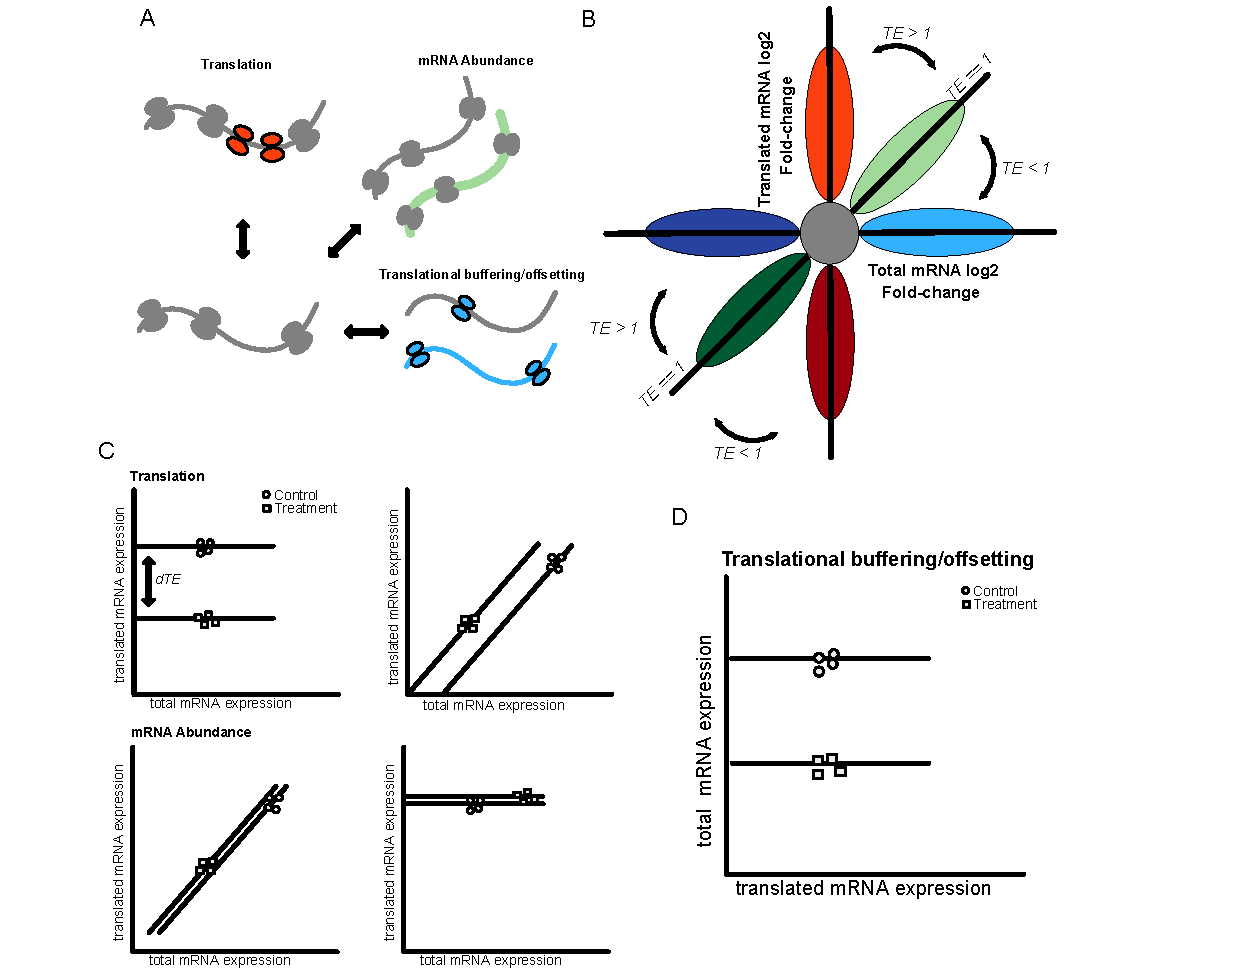
\includegraphics{./figures/geneModes.pdf}
  \caption{Regulatory modes of gene expression - A) simplifed overview. B) Schematic representation of regulatory modes of translation efficiency in a fold-change scatter plot. C) Schematic representation of the regulatory modes of translation efficiency data in anota2seq models. \label{geneModes}}
\end{figure}

\subsection{Algorithms for analysis of changes in Translational Efficiencies}

Initial approaches for analysis of transcriptome-wide translation
studies used an approach called the translation efficiency (TE-score).
This score calculates the ratio of the ratios between
polysome-associated mRNA levels divided by total mRNA levels within each
condition. The TE- score approach has been shown to be prone to spurious
correlations. The ratio of polysome-associated mRNA and total mRNA can
systematically correlate with total mRNA levels and thereby lead to
elevated false positive findings. Over the recent years several
algorithms to analyze polysome-profiling and ribosome-profiling data
have been developed these include babel (91), DESeq2 (92), RiboDiff
(93), Xtail (94). Although these methods have their distinct approach to
identify changes in translation efficiencies, their principle of
analysis is similar to comparing a ratio of ratios. Therefore these
methods suffer from similar issues as the TE-score. Another downside for
ratio of ratios-based methods is their inability to separate changes in
translational efficiencies altering protein levels from translational
buffering as any change in the nominator or denominator of any ratio
will implicate a difference in the ratio regardless of its origin. The
ANalysis Of Translational Activity (anota) (95) algorithm follows a
regression-based approach which couples analysis of partial variance
(APV or ANCOVA) (96) with the random variance model (RVM)(97). This
approach does not suffer from spurious correlations. The anota algorithm
was initially developed for analysis of DNA-microarray data, more
recently the anota algorithm has been adapted to accommodate data from
RNA-sequencing and released as anota2seq (76). During the development of
anota2seq the anota algorithm was e.g.~adapted to enable the user to
statistically separate multiple regulatory modes of gene expression
including changes in translation as well as translational buffering.
Thus, anota2seq allows for efficient interrogation of the translatome
without being affected by spurious correlations (76).

\chapter{Aims of this thesis}

The aims of this thesis are to explore the regulation of gene expression
in cancer, more specifically we investigate perturbations of gene
expression in different cancer models as a response to drug treatment.

In \textbf{Study I} we adapted an algorithm for ANalysis Of Translation
Activity data (anota) so that it could be applied to next generation
sequencing data. The resulting algorithm was named anota2seq.

We then applied the anota2seq algortihm to invesitigate changes in
translation efficiencies in two cancer models:

In \textbf{Study II} we unravelled the effects of eIF4A, an RNA
helicase, inhibition using a synthetic rocaglate CR-1-31-B (CR-31) in
pancreatic ductal adenocarcinoma.

In \textbf{Study III} we explored the effects of insulin on gene
expression in a breast cancer cell line.

\chapter{Results and discussion}

\chapter{Conclusions}

\chapter*{Acknowledgments}\label{acknowledgments}
\addcontentsline{toc}{chapter}{Acknowledgments}

Christina is awesome.

I am sorry for all the other people of this page but no one else helped
me more than my 8 paws of awesomeness Felix and Dexter. These little
litter shitters have been an extreme joy to be around and kept me sane
during the insanity that is writing a thesis. \textbf{Meow}

\chapter*{References}\label{references}
\addcontentsline{toc}{chapter}{References}

\hypertarget{refs}{}
\hypertarget{ref-Buttgereit1995}{}
Buttgereit, F., \& Brand, M. D. (1995). A hierarchy of ATP-consuming
processes in mammalian cells. \emph{The Biochemical Journal}, \emph{312
( Pt 1)}(Pt 1), 163--7. \url{https://doi.org/10.1042/bj3120163}

\hypertarget{ref-Carayol2008}{}
Carayol, N., Katsoulidis, E., Sassano, A., Altman, J. K., Druker, B. J.,
\& Platanias, L. C. (2008). Suppression of programmed cell death 4
(PDCD4) protein expression by BCR-ABL-regulated engagement of the
mTOR/p70 S6 kinase pathway. \emph{The Journal of Biological Chemistry},
\emph{283}(13), 8601--10. \url{https://doi.org/10.1074/jbc.M707934200}

\hypertarget{ref-Deragon2015}{}
Deragon, J.-M., \& Bousquet-Antonelli, C. (2015). The role of LARP1 in
translation and beyond. \emph{Wiley Interdisciplinary Reviews. RNA},
\emph{6}(4), 399--417. \url{https://doi.org/10.1002/wrna.1282}

\hypertarget{ref-Dever2012}{}
Dever, T. E., \& Green, R. (2012). The elongation, termination, and
recycling phases of translation in eukaryotes. \emph{Cold Spring Harbor
Perspectives in Biology}, \emph{4}(7), 1--16.
\url{https://doi.org/10.1101/cshperspect.a013706}

\hypertarget{ref-Fonseca2014}{}
Fonseca, B. D., Smith, E. M., Yelle, N., Alain, T., Bushell, M., \&
Pause, A. (2014). The ever-evolving role of mTOR in translation.
\emph{Seminars in Cell \& Developmental Biology}, \emph{36}, 102--112.
\url{https://doi.org/10.1016/j.semcdb.2014.09.014}

\hypertarget{ref-Fonseca2015}{}
Fonseca, B. D., Zakaria, C., Jia, J.-J., Graber, T. E., Svitkin, Y.,
Tahmasebi, S., \ldots{} Damgaard, C. K. (2015). La-related Protein 1
(LARP1) Represses Terminal Oligopyrimidine (TOP) mRNA Translation
Downstream of mTOR Complex 1 (mTORC1). \emph{The Journal of Biological
Chemistry}, \emph{290}(26), 15996--6020.
\url{https://doi.org/10.1074/jbc.M114.621730}

\hypertarget{ref-Gandin2016a}{}
Gandin, V., Masvidal, L., Cargnello, M., Gyenis, L., McLaughlan, S.,
Cai, Y., \ldots{} Topisirovic, I. (2016). mTORC1 and CK2 coordinate
ternary and eIF4F complex assembly. \emph{Nature Communications},
\emph{7}(1), 11127. \url{https://doi.org/10.1038/ncomms11127}

\hypertarget{ref-Hanahan2011}{}
Hanahan, D., \& Weinberg, R. A. (2011). Hallmarks of cancer: The next
generation. \emph{Cell}, \emph{144}(5), 646--674.
\url{https://doi.org/10.1016/j.cell.2011.02.013}

\hypertarget{ref-Hay2004}{}
Hay, N., \& Sonenberg, N. (2004). Upstream and downstream of mTOR.
\emph{Genes \& Development}, \emph{18}(16), 1926--1945.
\url{https://doi.org/10.1101/gad.1212704}

\hypertarget{ref-Hinnebusch2014}{}
Hinnebusch, A. G. (2014). The scanning mechanism of eukaryotic
translation initiation. \emph{Annual Review of Biochemistry}, \emph{83},
779--812. \url{https://doi.org/10.1146/annurev-biochem-060713-035802}

\hypertarget{ref-Hsieh2010}{}
Hsieh, A. C., Costa, M., Zollo, O., Davis, C., Feldman, M. E., Testa, J.
R., \ldots{} Ruggero, D. (2010). Genetic Dissection of the Oncogenic
mTOR Pathway Reveals Druggable Addiction to Translational Control via
4EBP-eIF4E. \emph{Cancer Cell}, \emph{17}(3), 249--261.
\url{https://doi.org/10.1016/j.ccr.2010.01.021}

\hypertarget{ref-Laplante2012}{}
Laplante, M., \& Sabatini, D. M. (2012). mTOR Signaling. \emph{Cold
Spring Harbor Perspectives in Biology}, \emph{4}(2), a011593.
\url{https://doi.org/10.1101/cshperspect.a011593}

\hypertarget{ref-Leibovitch2018}{}
Leibovitch, M., \& Topisirovic, I. (2018). Dysregulation of mRNA
translation and energy metabolism in cancer. \emph{Advances in
Biological Regulation}, \emph{67}, 30--39.
\url{https://doi.org/10.1016/j.jbior.2017.11.001}

\hypertarget{ref-Magnuson2012}{}
Magnuson, B., Ekim, B., \& Fingar, D. C. (2012). Regulation and function
of ribosomal protein S6 kinase (S6K) within mTOR signalling networks.
\emph{Biochemical Journal}, \emph{441}(1), 1--21.
\url{https://doi.org/10.1042/BJ20110892}

\hypertarget{ref-Oh2010}{}
Oh, W. J., Wu, C. c., Kim, S. J., Facchinetti, V., Julien, L. A.,
Finlan, M., \ldots{} Jacinto, E. (2010). mTORC2 can associate with
ribosomes to promote cotranslational phosphorylation and stability of
nascent Akt polypeptide. \emph{The EMBO Journal}, \emph{29}(23),
3939--3951. \url{https://doi.org/10.1038/emboj.2010.271}

\hypertarget{ref-Pearce2007}{}
Pearce, L. R., Huang, X., Boudeau, J., Pawłowski, R., Wullschleger, S.,
Deak, M., \ldots{} Alessi, D. R. (2007). Identification of Protor as a
novel Rictor-binding component of mTOR complex-2. \emph{Biochemical
Journal}, \emph{405}(3), 513--522.
\url{https://doi.org/10.1042/BJ20070540}

\hypertarget{ref-Roux2012}{}
Roux, P. P., \& Topisirovic, I. (2012). Regulation of mRNA translation
by signaling pathways. \emph{Cold Spring Harbor Perspectives in
Biology}, \emph{4}(11), a012252.
\url{https://doi.org/10.1101/cshperspect.a012252}

\hypertarget{ref-Roux2018}{}
Roux, P. P., \& Topisirovic, I. (2018). Signaling Pathways Involved in
the Regulation of mRNA Translation. \emph{Molecular and Cellular
Biology}, \emph{38}(12). \url{https://doi.org/10.1128/MCB.00070-18}

\hypertarget{ref-Saxton2017}{}
Saxton, R. A., \& Sabatini, D. M. (2017). mTOR Signaling in Growth,
Metabolism, and Disease. \emph{Cell}, \emph{168}(6), 960--976.
\url{https://doi.org/10.1016/j.cell.2017.02.004}

\hypertarget{ref-Schepetilnikov2013}{}
Schepetilnikov, M., Dimitrova, M., Mancera-Martínez, E., Geldreich, A.,
Keller, M., \& Ryabova, L. A. (2013). TOR and S6K1 promote translation
reinitiation of uORF-containing mRNAs via phosphorylation of eIF3h.
\emph{The EMBO Journal}, \emph{32}(8), 1087--1102.
\url{https://doi.org/10.1038/emboj.2013.61}

\hypertarget{ref-Tcherkezian2014}{}
Tcherkezian, J., Cargnello, M., Romeo, Y., Huttlin, E. L., Lavoie, G.,
Gygi, S. P., \& Roux, P. P. (2014). Proteomic analysis of cap-dependent
translation identifies LARP1 as a key regulator of 5'TOP mRNA
translation. \emph{Genes \& Development}, \emph{28}(4), 357--371.
\url{https://doi.org/10.1101/gad.231407.113}

\hypertarget{ref-Wang2001}{}
Wang, X., Li, W., Williams, M., Terada, N., Alessi, D. R., \& Proud, C.
G. (2001). Regulation of elongation factor 2 kinase by p90(RSK1) and p70
S6 kinase. \emph{The EMBO Journal}, \emph{20}(16), 4370--9.
\url{https://doi.org/10.1093/emboj/20.16.4370}

\hypertarget{ref-Wurth2015}{}
Wurth, L., \& Gebauer, F. (2015). RNA-binding proteins, multifaceted
translational regulators in cancer. \emph{Biochimica et Biophysica
Acta}, \emph{1849}(7), 881--6.
\url{https://doi.org/10.1016/j.bbagrm.2014.10.001}

\hypertarget{ref-Yang2003}{}
Yang, H.-S., Jansen, A. P., Komar, A. A., Zheng, X., Merrick, W. C.,
Costes, S., \ldots{} Colburn, N. H. (2003). The transformation
suppressor Pdcd4 is a novel eukaryotic translation initiation factor 4A
binding protein that inhibits translation. \emph{Molecular and Cellular
Biology}, \emph{23}(1), 26--37.
\url{https://doi.org/10.1128/mcb.23.1.26-37.2003}

\end{document}
